%----------------------------------------------------------------------------------------
%	PACKAGES AND OTHER DOCUMENT CONFIGURATIONS
%----------------------------------------------------------------------------------------

\documentclass[twoside,fontsize=10pt]{article}
%\documentclass[oneside]{article}
\usepackage{lipsum} % Package to generate dummy text throughout this template
\usepackage{graphicx}

%\usepackage[sc]{mathpazo} % Use the Palatino font
\usepackage[T1]{fontenc} % Use 8-bit encoding that has 256 glyphs
%\linespread{1.05} % Line spacing - Palatino needs more space between lines
\usepackage{microtype} % Slightly tweak font spacing for aesthetics
\usepackage{listings}
\usepackage[hmarginratio=1:1,top=32mm,columnsep=20pt]{geometry} % Document margins
%\usepackage{multicol} % Used for the two-column layout of the document
\usepackage[hang, small,labelfont=bf,up,textfont=it,up]{caption} % Custom captions under/above floats in tables or figures
\usepackage{booktabs} % Horizontal rules in tables
\usepackage{float} % Required for tables and figures in the multi-column environment - they need to be placed in specific locations with the [H] (e.g. \begin{table}[H])
\usepackage[hidelinks]{hyperref} % For hyperlinks in the PDF

\usepackage{lettrine} % The lettrine is the first enlarged letter at the beginning of the text
\usepackage{paralist} % Used for the compactitem environment which makes bullet points with less space between them
\usepackage{chngcntr}
\counterwithout{figure}{section}
\usepackage{abstract} % Allows abstract customization
\renewcommand{\abstractname}{}    % clear the title
\renewcommand{\absnamepos}{empty}
\renewcommand{\abstractnamefont}{\normalfont\bfseries} % Set the "Abstract" text to bold
\renewcommand{\abstracttextfont}{\normalfont\small\itshape} % Set the abstract itself to small italic text
\usepackage[super, sort&compress]{natbib}
\setlength{\bibsep}{0.0pt}
\bibliographystyle{unsrtnat}
\usepackage{titlesec} % Allows customization of titles
\renewcommand\thesection{\Roman{section}} % Roman numerals for the sections
\renewcommand\thesubsection{\Roman{subsection}} % Roman numerals for subsections
\titleformat*{\section}{\LARGE\scshape\centering}
\renewcommand{\bibsection}{\section*{\refname}}
\titleformat{\section}[block]{\LARGE\scshape\centering}{\thesection}{1em}{} % Change the look of the section titles
\titleformat{\subsection}[block]{\large\bfseries}{\thesubsection}{1em}{} % Change the look of the section titles
\titleformat{\subsubsection}[block]{\bfseries\textit}{\thesubsubsection}{0.1mm}{} % Change the look of the section titles
\usepackage[table,xcdraw]{xcolor}
\usepackage{caption}


\usepackage{fancyhdr} % Headers and footers
\pagestyle{fancy} % All pages have headers and footers
\fancyhead{} % Blank out the default header
\fancyfoot{} % Blank out the default footer
\fancyhf{}
\renewcommand{\headrulewidth}{0pt}
%\fancyhead[C]{Running title $\bullet$ November 2012 $\bullet$ Vol. XXI, No. 1} % Custom header text
\fancyfoot[RO,LE]{\thepage} % Custom footer text

%----------------------------------------------------------------------------------------
%	TITLE SECTION
%----------------------------------------------------------------------------------------

\title{\vspace{-15mm}\fontsize{18pt}{10pt}\normalfont\textbf{Everything should be linked: linking and visualising data for dynamic  multidimensional biological data interpretation.\\ \vspace{4 mm} {{\footnotesize \textit{Exploring multi-level effects of structural variations in non-coding genomic regions in cancer}}}}} % Article title

\author{
\large
\textsc{RHWE (Robin) van der Weide}\thanks{Supervisor: Joep de Ligt, PhD}\\[2mm] % Your name
\normalsize   Cancer Stem cells \& Developmental biology \\ % Your institution
\normalsize  Utrecht Graduate School of Life Sciences \\ % Your institution
%\normalsize \href{mailto:john@smith.com}{john@smith.com} % Your email address
\vspace{-5mm}
}
\date{}

%----------------------------------------------------------------------------------------

\begin{document}

\maketitle % Insert title

\thispagestyle{fancy} % All pages have headers and footers

%----------------------------------------------------------------------------------------
%	ABSTRACT
%----------------------------------------------------------------------------------------
\newpage
\mbox{   }
\newpage
\renewcommand{\abstractname}{\begin{center}
Summary of the research
\end{center}}    % clear the title
\begin{abstract}
\noindent
To date, studies on non-coding regions of the genome, specifically in cancer, have been limited. This is mainly due to the complex nature of putative functional elements in these regions. In parallel with the ENCODE-project, the interest in these regions has increased: researchers are beginning to study causal non-coding variations in cancer\cite{Benko2009,Kurth2009}. Due to the increase in popularity and cost-effectiveness of various omics-approaches, more and more data is becoming available. The complexity of integrating and analysing information of these approaches increases with every added omics-layer and/or dimension (e.g. time-series, treatments). When studying the consequences of structural variants in non-coding regions in cancer, this complexity is further increased due to cancer-specific (e.g. heterogeneous samples, rapid evolution) and structural variant-specific (e.g. multiple types and consequences) factors.
\medskip

\noindent
The current methods for integrating and analysing these layers and dimensions have two major limitations in their design: scalability and generality (i.e. the possibility to add more levels and/or dimensions). Moreover, there isn't an option to overview a dataset without filtering, dividing or restructuring the data. These limitations restrict the integration of complex datasets, which is needed to truly understand the complex biology of cancer\citet{Munoz2011}.
\medskip

\noindent Enter the Semantic Web and its Resource Description Framework (RDF). A simple and flexible framework for describing anything about anything.
% An example of such a RDF-instance (a triple) is "BRAF1 has the molecular function of binding calcium ion", which has these three parts: a subject (BRAF1), a predicate (molecular function) and an object (binding calcium ion). Another triple can then say something about the phosphorylated protein levels of this gene in a sample. Connecting these two triples would enable a researcher to find a possible pattern in the data (i.e. a gene, responsible for calcium ion binding, has a low phosphorylation level in the investigated sample). 
Since every type of data can be translated to this universal language, integration of large datasets of different levels and dimensions becomes possible and a lot more feasible. When researchers have translated their local data to RDF, they can easily connect and combine it with public repositories (EMBL-EBI has already launched six databases, including UniProt and Reactome), which makes analyses even more powerful. By using the SPARQL Protocol and RDF Query Language (SPARQL), retrieving and manipulating data in RDF is easily readable by both humans and computers. The SPARQL-results can subsequently be visualized as a whole, or filtered by the user. 
\medskip

\noindent Here, we propose the use of semantic web technologies and visual analytics to decrease the complexity of integrating and visualizing multi-level and -dimensional biological data, thereby enabling further elucidation of the complex biology of, for example, cancer. Firstly, we will create the framework needed to design the missing tools for converting the most-used NGS-formats to RDF. Next, visualisations (based on visual analytics) of the biological RDF-data will be created, which will be used to perform previously impossible integration-focussed analyses on the consequences of structural variation in the non-coding regions of cancer-genomes.
\end{abstract}
\medskip
\renewcommand{\abstractname}{\begin{center}
Layman's summary
\end{center}}    % clear the title
\begin{abstract}\noindent
The biomedical research community wants to be able to combine and analyse a multitude of biological signals in one experiment, because the biology of, for example, cancer is so complex. However, integrating diverse sets of biological signals is currently a major challenge. To overcome this, we propose the use of Semantic Web-methods: these are specifically designed for integrating vast amounts of different data. Furthermore, it allows users to describe, analyse and test their data interactively and dynamically via visual representations displayed in the browser. 

Research on non-coding genomic regions, for example, would benefit greatly from these methods. It would enable studies on the complex cancer-causing consequences of changes in parts of chromosomes that do not contain a gene.

A preliminary study shows the added value of such methods in biology: researchers are able to describe, analyse and test 20 times more biological questions in the same time, compared to conventional methods. We propose to develop these methods further for the research-community (and biology in particular), enabling us to perform research on variations in the non-coding genomic regions in cancer. \\
\medskip

\noindent \textbf{Keywords:} structural variation, multi-level data integration, next-generation sequencing, cancer, visual analytics
\end{abstract}



%----------------------------------------------------------------------------------------
%	ARTICLE CONTENTS
%----------------------------------------------------------------------------------------
\newpage
\section*{Background, aims and approach}
\subsection*{Overall aim}
The aim of this project is to integrate and visualise multiple levels and dimensions of (NGS-based) omics-data with methods of the semantic web and, using these methods, further understand the consequences of structural variations in the non-coding regions of the genome on other biological levels, like the transcriptome and proteome. Thus, this proposal has three sub-projects, which rely heavily on each other:

\begin{enumerate}
\item \textbf{Data-integration} 
Integration of NGS-based data by using Semantic Web-methodologies to improve integrative bioinformatics in general and NGS-based multi-level and -dimensional research in particular.
\item \textbf{Visual analytics} 
Linking the Semantic-Web data to D3.js, enabling us to dynamically and interactively visualise RDF-data.
\item \textbf{Multi-level analysis} 
Multi-level and -dimensional integrative bioinformatical analysis to elucidate the consequences of genomic structural variations in non-coding regions in cancer.
\end{enumerate}
\subsection*{Scientific relevance and challenges} % inleiding: complex bio at the moment/problemen stellen (eindigen met "in this proposal, Will.. etc)
%=================================================
%=================================================
%Explain the importance of the problem or critical barrier to progress in the field that the proposed project addresses.
%Explain how the proposed project will improve scientific knowledge, technical capability, and/or clinical practice in one or more broad fields.
%Describe how the concepts, methods, technologies, treatments, services, or preventative interventions that drive this field will be changed if the proposed aims are achieved.
%=================================================
%=================================================
%stukje over cancer%Moreover, there already have been successfully studies, linking non-coding regions to colorectal- and skin-cancer\cite{Ongen2014,Huang2013}. 
The majority of genomics studies are focussed on finding causal genetic variation in the protein-coding regions of the genome. However, these regions amount only to approximately two percent\cite{Lander2001}. One of the major reasons behind this is the relative uncomplicated nature of studying coding regions, as consequences on lower levels (e.g. transcription, proteins) are traceable\cite{McLaren2010}. This is in contrast to the non-coding regions, which often do not show a linear effect on other levels\cite{Bird2006}. A good illustration of the complexity of the non-coding regions is the ENCyclopedia Of DNA Elements (ENCODE)-project\cite{ENCODE}, which contains over fifty different signals (e.g. histone methylation, DNase1 hypersensitivity). 

The fact that non-coding regions often have roles in regulation of a distant genes (i.e. cis-acting), provides even more complexity to the analysis of structural variants (SVs) in these regions. For example the Pierre Robin Syndrome (PRS): structural variations (deletions or duplications) in the 3Mb surrounding the SOX9-gene in specific tissues, are causative of the striking phenotype of undeveloped mandibles and tongue in children\cite{Benko2009,Kurth2009}. Studies on cancer-specific causative non-coding variation are beginning to emerge in the last two years, including colorectal- and skin-cancer\cite{Ongen2014,Huang2013}, and computational methods for non-coding regions are just starting to come up in the literature of 2014\cite{Khurana2013,Kircher2014}.  
\medskip

\noindent
The amount of (public) biological data has exploded in the last years (even outpacing Moore's law\footnote{A two-fold in- or decrease of a variable (here: dollar/nt) per two years.}) which is the result of the advances in omics-technologies like Next-Generation Sequencing (NGS) and Mass-Spectrometry (MS), in both performance and costs. Aside from the sheer size, a second factor for the highly complex nature of current biomedical research is the addition of other dimensions, like time-series or treatments to the aforementioned omics-levels and other types of data from the same level. While there are plenty of studies on single-level data analysis, both academia and industry agree that data-integration is key to understanding the complex nature of biology more thoroughly \citep{Gomez-Cabrero2014, Huttenhower2010, Searls2005, Hamid2009}. 

However, only a few layers and/or dimensions have been integrated per study and results are -for the most part- cherry picked, instead of fully systematic. This is mainly due to the methods used in integration-studies, which are limited due to the large amounts of parsing-time (i.e. the time to convert various file/region-formats): most of them are set up in the same manner as individual-level experiments, whereafter they are combined. These methods cause high amounts of analytical time, as was the case in the study of \citet{Munoz2011}: every two months of data-accumulation costed two years of analysis. The limited number of truly integrative studies use computational approaches to reconstruct biological networks. While this is a valid strategy, scaling the analysis from the bacteria used by \citet{Karr2012} and \citet{Lerman2012} to multi-cellular organisms proves to be difficult. The most obvious reasons for this are the complexity of the used mathematical methods, the integration of multiple data-sources (with varying file-formats) and/or the use of a inflexible database-structures. 
\medskip

\noindent
To overcome these scaling issues, \textbf{we propose the use of the Semantic Web: the \textit{Resource Description Framework} (RDF) and its query-language \textit{SPARQL Protocol and RDF Query Language} (SPARQL)}. RDF is a general and simple framework for making statements about subjects, already heavily used in fields outside of biology, enabling users to integrate and search data based on semantics. Within biology, RDF is only used sparsely and mainly focussed on external data-source integration and not on own data \cite{Belleau2008,Neumann2006,Sahoo2008}. Every RDF-statement (i.e. a triple) has three parts: a subject, a predicate and an object (e.g. \lstinline|BRAF1 :: molecular function :: calcium ion binding|). This makes it possible to link every object to another and denote the relationship between them: no additional (file)formats are needed (fig.\ref{fig:rdf}). 

Compared to other relational database management systems, RDF is completely flexible: no database-schemas (pre-specified structures for the data, like the mySQL-method of \citet{Low2013}) are needed. Aside from the non-complex, flexible and self-describing nature of the RDF-data, triples can be seen as a modular directed graph: users can combine multiple relevant RDF-sources (e.g. UniProt and/or Proteomics-data). Every additional RDF-source results in a more relevant and heterogeneous population of triples, making the network more complex and informative. Extracting relevant information from this "hairball" of linked objects and subjects has been a major issue and challenge since the beginning of big data, as \citet{Pavlopoulos2008} stated in 2008. SPARQL provides the ability to filter on an arbitrary number of (human-readable) expressions and can combine multiple databases to query, like the RDF-databases of EMBL-EBI \citep{Jupp2014}. Another advantage of using SPARQL is the increase in scalability by including multiple triplestores in the same query. Such a federated query results in faster retrieval of the data, by enabling the use of small, specific triplestores.

\medskip
\begin{figure}[H]
    \centering
    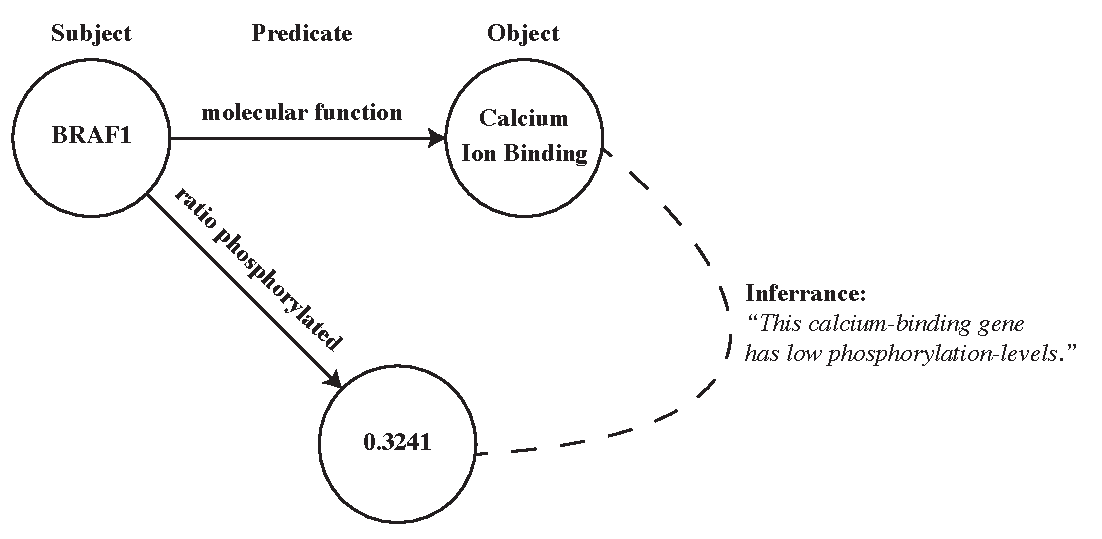
\includegraphics[width=0.75\textwidth]{rdf}
    \caption{\textbf{General outline of RDF.} By linking two triples by their common subjects, one can infer the relationship between the two objects via the predicates and find patterns: a gene, responsible for calcium ion binding, has a low phosphorylation level in the investigated sample.}
    \label{fig:rdf}
\end{figure}
\noindent
When data is integrated in a Semantic Web RDF-database (TripleStore) and a relevant set of subjects, predicates and/or objects are extracted using SPARQL, the remaining dataset is still very large. The abstract and complex nature of this "hairball" makes it hard to formalise an analytical problem to solve. \textbf{To create interactive and dynamic visual representations of a dataset, we propose to use of the multidisciplinary theories and methods of \textit{visual analytics}}. \citet{Thomas2005} describe this field in 2005 as "\textit{the science of analytical reasoning facilitated by interactive visual interfaces.}". It uses analytical and statistical methods from fields as computer science and statistics and visualisation-techniques from cognitive and design sciences. This enables effective (exploratory) analysis of the data by the user. Drug discovery is one of the leading fields in biological visual analytics, as it provides a more cost-effective method for analysing data of clinical trails\cite{Cao2008}.

The JavaScript library Data Driven Documents (\textit{D3.js}) is well suited for implementing linked data -which itself is already a graph- within visual analytics, as it is focussed on structuring data for dynamic, web-base visualisations(using current standards like HTML \& SVG)\cite{Bostock2011}. And since it is embedded in HTML, additional operators (e.g. buttons, SPARQL-forms) can be added. Due to these benefits, the use of D3.js in visual analytics is increasing: a notable biology-specific example of this is Epiviz2\cite{Chelaru2014}. However, this tool only takes a specific set of data-formats and -levels and -more importantly- only shows a specific genomic region, instead of the complete scope. This can easily lead to "\textit{cherry picking}", instead of data-focussed formulation and analysis of hypotheses.
\medskip

\noindent 
The heterogeneous samples and datasets of cancer make it one of the most computationally demanding types of integrative biology. \textbf{We propose to use our methods to study to consequences of structural variations at non-coding loci in cancer on other levels.}  These methods will enable research in this technical challenging topic, by decreasing the computational burden of data-handling, and increase the cognitive abilities of the user, by providing integrative visual interfaces. 



%Usage case: structural variants of non-coding regions in cancer
%twee dingen zeker noemen: hetrrogeneous dataset en de complicaties van multiu-level en dimensional in kanker-onderzoek
%

%\cite{Gomez-Cabrero2014} geeft mooie inleiding (en over de wensen van de community)


\subsection*{Originality and innovative character} 
%=================================================
%=================================================
%Explain how the application challenges and seeks to shift current research or clinical practice paradigms.
%Describe any novel theoretical concepts, approaches or methodologies, instrumentation or interventions to be developed or used, and any advantage over existing methodologies, instrumentation, or interventions.
%Explain any refinements, improvements, or new applications of theoretical concepts, approaches or methodologies, instrumentation, or interventions.
%=================================================
%=================================================
The 2014 survey of \citet{Gomez-Cabrero2014} showed that biomedical academics had the highest interest (78.2 percent) in the integration of multiple omics-datasets and that there was a high need for standardized tools and data-types. Especially data-storage, -exploration and -exploitation were found the be key: their conclusions were best summarized by \textit{the need for having exploration tools, which combine summery statistics and interactive visualisations, to analyse heterogeneous data-sets}.
\medskip

\noindent
There have been various studies on integration of biological signals with the aid of semantic web technologies, as the power of ontology-based entailment\footnote{The logical consequence of having two linked ontologies, thereby inferring an additional, encompassing relationship on the shared object/subject} reasoning is widely acknowledged\cite{Sahoo2008}. However, the momentum was lacking: until 2014, big databases were not available in RDF-format. This meant that bioinformatical research involving RDF had little to no outside support, as they could only integrate their own data, like the integration of RDF-methods in microarray analyses by \citet{Szpakowski2009} in 2009. Recently, EMBL-EBI has opened their own RDF-platfom, boasting six big data-sources (Gene Expression Atlas, ChEMBL, BioModels, Reactome, BioSamples and UniProt)\cite{Jupp2014}. This was the boost needed to further incorporate RDF in biological analyses.

However, there are two main limitations of this relatively young incorporation: a standard language for denoting biological triples (e.g. chromosome locations) is missing and the focus lies at linking database-accessions \citep{Ruttenberg2007}. While the first limitation could also be a strength (everybody can use their own dialect), a standardisation-step will lower the learning-curve, which will enable researchers in all fields of biology to fully benefit from the integrative benefits of the Semantic Web. The second limitation is  severely restricting the use of RDF in NGS- and MS-based methods: there are no tools to convert the common formats, like the \textit{Variant Call Format} (VCF) and \textit{Sequence Alignment Format} (SAM), to triples. An example of this is  \textit{Bio2RDF}\cite{Belleau2008}: a "\textit{RDFizer}", which converts common databases, like the ones from NCBI, to triplestores. One of the main innovative points of our proposal is the development of methods to handle the NGS- and MS-based formats for use in the Semantic Web. This will result in a broader use of semantic web-technologies for the research community, by enabling the coupling of proprietary NGS- and MS-data to existing RDF-databases.
\medskip

\noindent
%added value of linked data visual analytics TOV standaard methodes ( verwijs naar pilot study)
The implementation of web-based visual analytics for RDF-databases is another major innovative point in this proposal. Combining Semantic Web-technology with this will create a paradigm shift in the way integrative analysis of (biological) data is done. Visual analytics have been shown to result in the most optimal analysis-effectivity, as it allows the user to combine the data with their own background and intuition (fig. \ref{fig:ae}). Not only can data be more effectively analysed, but it can also be better understood and presented, due to the ability to provide an overview of the complete dataset \cite{Thomas2005, Keim}. 

\begin{figure}[H]
    \centering
    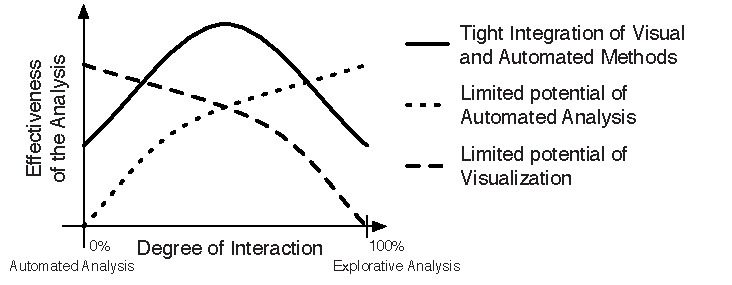
\includegraphics[width=0.75\textwidth]{autoVSexplo}
    \caption{\textbf{Trade-offs between automated and explorative analysis.} By combining automated analyses, where appropriate, with the background and intuition of the user, an optimal amount of effectivity can be attained. Picture taken from \citet{Keim}.}
    \label{fig:ae}
\end{figure}
\medskip

\noindent
While there has already been a large amount of work in the field of computational cancer research, the vast majority of large-scale integrative studies have been performed on the coding-regions (which account for 2 percent of the total size) of the genome\cite{ENCODE}. Genome-Wide Association Studies (GWASs) on a broad range of (hereditary) cancer-types have shown, that non-coding locations are associated with these diseases. Until 2013, however, tools and sources to find the precise causative variations in non-coding genomic regions were limited. In the last two years, several advances have made it possible to asses the consequences of individual variations in non-coding regions\cite{Ongen2014,Khurana2013}, but no large-scale integrative studies have been performed (partly due to the current state of integrative methods). 

Due to the affiliation with the University Medical Center Utrecht (UMCU), we are in the unique position to test our hypotheses and methods in both research and clinical settings. Furthermore, the HUB-biobank in the Hubrecht Institute enables us to also perform analyses on organoids, providing us a stable and homogeneous \textit{in vitro} platform for (validation-)studies on cancer-samples. With the new methods, we will be in the position to perform fully integrative studies on the underlying mechanisms and consequences of (structural) variation in cancer.

\subsection*{Pilot-study}
To asses to feasibility of our proposal, a small-scale pilot-study was performed on de data of \citet{VanHeesch2014}. This dataset includes transcriptome data of mRNA's, bound to a number of ribosomal units (1 to 7+) and matching exome-data. If one would be interested to look at the molecular functions of a gene, which transcripts have a bias for one allele, a disproportional amount of time is lost on parsing, intersecting and downloading various types of data (fig. \ref{fig:awesome_image}). With the current methods, twelve set-operations (e.g. intersections, unions) have to be performed on approximately 5gb of data and three datasets ($\pm$15gb) have to be completely downloaded (once, until a new version is launched) before a simple exploratory question can be answered. Approximately three and a half hours was needed to perform this, in contrast to one hour with our methods. Of this hour, more than fifty minutes were used to convert VCF to RDF and load the 4store database: every query hereafter takes up approximately 10 minutes. This pilot illustrates two important factors: the low-complex nature of the proposed methods and the valuable property of having a separate query-stage, which results in being able to make more than ($\frac{(8*60)-50}{10}= $) forty queries in eight hours, instead of approximately ($\frac{8-3,5}{3,5}= $) two queries with the currently used methods.

\begin{figure}[H]
    \centering
    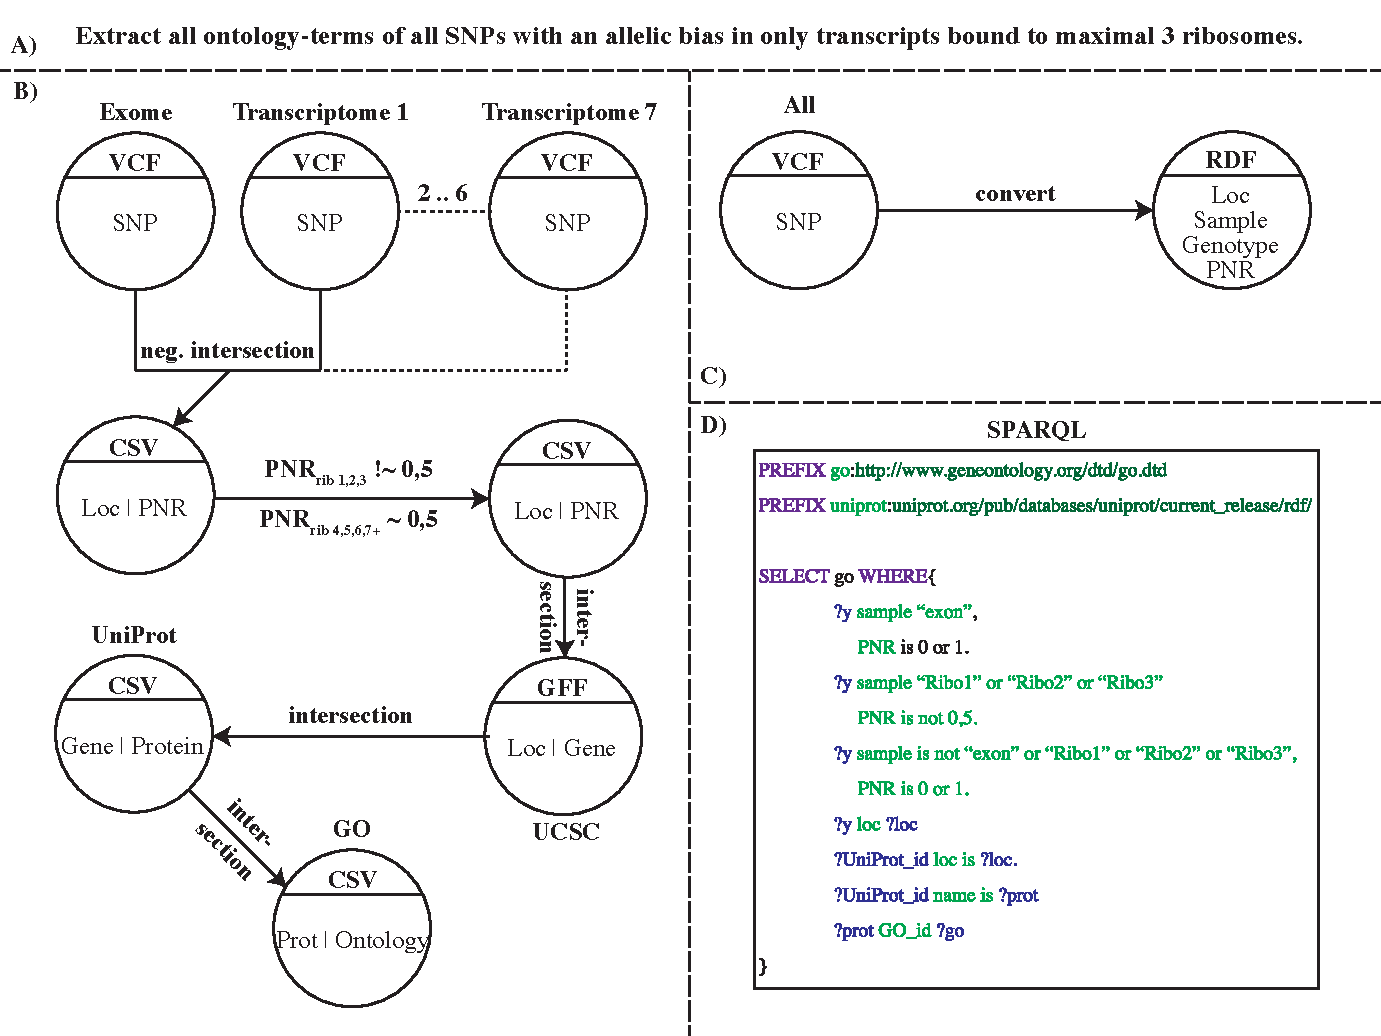
\includegraphics[width=0.75\textwidth]{DifferencesInDoingThings}
    \caption{\textbf{Differences between current integration techniques and RDF.} When a researcher has a question like \textbf{A}, they have to go through a series of parsing and interception steps, like in \textbf{B}. External sources have to be fully downloaded and converted, before use. Our proposed pipeline (shown in \textbf{C}), firstly converts the data to RDF. Then, a question can be formulated in SPARQL (\textbf{D}), incorporating relevant outside sources, which can be easily changed without having to juggle/download the data again.}
    \label{fig:awesome_image}
\end{figure}
\subsection*{Methods and techniques} %M&M
%=================================================
%=================================================
%Describe the overall strategy, methodology, and analyses to be used to accomplish the specific aims of the project. Include how the data will be collected, analyzed, and interpreted as well as any resource sharing plans as appropriate.
%Discuss potential problems, alternative strategies, and benchmarks for success anticipated to achieve the aims.
%As applicable, also include the following information as part of the Research Strategy, keeping within the three sections listed above: Significance, Innovation, and Approach.
%=================================================
%=================================================
Data acquisition will be performed throughout the study. Ongoing sequencing efforts from the research group of Prof. Dr. Cuppen and collaborators will ensure more than adequate amounts of data will be at our disposal. Due to the accompanied scientific questions of this data, the developmental stages of this study will continue to be focussed and inspired by the end-goal: answering biological questions. Furthermore, continuing the data-acquisition in the second half of the study to will enable us to collaborate with the research community and showcase our innovative technology with new and exciting integrative biology studies.
\medskip

\noindent
To ensure the greatest compatibility and effectiveness, tight collaborations will be established between leading RDF-users and -developers in- and outside of biology. Triples for NGS- and MS-based data will be developed, taking into account the most commonly used format first. Since different databases can require a specific triple-structure, RDF-databases will be investigated on their ability to handle the large datasets efficiently, including their in- and output options. Selected research groups in Utrecht will be attracted to provide early feedback-rounds, focussed on usability and compatibility. 

Once the triple-development of a data-format is completed (i.e. end-users and the RDF-community have provided positive feedback), development of the conversion-tools is next. In this stage, we seek to expand the capabilities of current leading bioinformatical tools like Sambamba\cite{Tarasov2014} and BIO-VCF\cite{Goto2010}, to capitalise on their multi-core capabilities. Furthermore, we will seek to collaborate with the current (public data-focussed) initiatives, like Bio2RDF\cite{Belleau2008} and BioInterchange\cite{Baran} to ensure software-compatibility and limit redundancy.
\medskip

\noindent
The visualisation-subproject will have two phases. In the first phase, we will use a minimalistic model -creating visual analytics-based solutions for the analysis of SNPs and transcript levels of associated genes- to develop the link between the SPARQL in- and output and \textit{d3.js}-visualisation. 

After a successful first phase, the second phase will broaden the available visualisations, by creating a modular dashboard. Every module will provide a specific visual (e.g. heatmap, scatterplot) and will interact with both the SPARQL-input, -output and with the other active modules. If a user would, for example, select a specific gene in the scatterplot, the same data-point will be highlighted in the other modules. The cross-talk between modules has already been implemented in Epiviz2\cite{Chelaru2014}, which is highly appraised for this by its users. The order of development of specific modules will be primarily based on the wants and needs of the community, which will be gathered with the above-mentioned feedback-rounds.
%\newpage
\section*{Research plan}
\subsection*{Timetable}
\begin{table}[h]
\begin{center}
\begin{tabular}{lllllllll}
                                                & \multicolumn{8}{c}{Semesters}                                                                                                                                                                                                                                                                                                                                                                                 \\ \cline{2-9} 
                                                & S1                                              & S2                                              & S3                                              & S4                                              & S5                                              & S6                                              & S7                                              & S8                                              \\ \hline
\textbf{Data acquisition}                       & \cellcolor[HTML]{343434}{\color[HTML]{656565} } & \cellcolor[HTML]{343434}{\color[HTML]{656565} } & \cellcolor[HTML]{343434}{\color[HTML]{656565} } & \cellcolor[HTML]{343434}{\color[HTML]{656565} } & \cellcolor[HTML]{343434}{\color[HTML]{656565} } & \cellcolor[HTML]{343434}{\color[HTML]{656565} } & \cellcolor[HTML]{343434}{\color[HTML]{656565} } & \cellcolor[HTML]{343434}{\color[HTML]{656565} } \\
\textbf{Aim 1: Data-integration}                & \cellcolor[HTML]{343434}                        & \cellcolor[HTML]{343434}                        & \cellcolor[HTML]{343434}                        &                                                 &                                                 &                                                 &                                                 &                                                 \\
\hspace*{1em} Developing omics-specific triples & \cellcolor[HTML]{656565}                        &                                                 &                                                 &                                                 &                                                 &                                                 &                                                 &                                                 \\
\hspace*{1em} Coding conversion-tools           &                                                 & \cellcolor[HTML]{656565}                        & \cellcolor[HTML]{656565}                        &                                                 &                                                 &                                                 &                                                 &                                                 \\
\hspace*{1em} Writing Best-Practices            &                                                 &                                                 & \cellcolor[HTML]{656565}                        &                                                 &                                                 &                                                 &                                                 &                                                 \\
\textbf{Aim 2: Visual analytics}                &                                                 &                                                 & \cellcolor[HTML]{343434}                        & \cellcolor[HTML]{343434}                        &                         \cellcolor[HTML]{343434}                                               &                                                 &                                                 &                                                 \\
\hspace*{1em} Coding SPARQL+D3 endpoint         &                                                 &                                                 & \cellcolor[HTML]{656565}                        &                                                 &                                                 &                                                 &                                                 &                                                 \\
\hspace*{1em} Adding visualisation-methods      &                                                 &                                                 & \cellcolor[HTML]{656565}                        & \cellcolor[HTML]{656565}                        &                                                 &                                                 &                                                 &                                                 \\
\hspace*{1em} Adding filtering and output       &                                                 &                                                 &                                                 & \cellcolor[HTML]{656565}                        &                                                \cellcolor[HTML]{656565}   &                                                 &                                                 &                                                 \\
\textbf{Aim 3: Multi-level analysis}            &                                                 &                                                 &                                                 &                                                 &  & \cellcolor[HTML]{343434}{\color[HTML]{343434} } & \cellcolor[HTML]{343434}{\color[HTML]{343434} } & \cellcolor[HTML]{343434}{\color[HTML]{343434} } \\
\hspace*{1em} Consequences of Cancer-SV's       &                                                 &                                                 &                                                 &                                                 &                        & \cellcolor[HTML]{656565}                        & \cellcolor[HTML]{656565}                        & \cellcolor[HTML]{656565}                        \\
\textbf{Writing thesis}                         &                                                 &                                                 &                                                 &                                                 &                                                 &                                                 &                                                 & \cellcolor[HTML]{343434}                       
\end{tabular}
\end{center}
\end{table}


\subsection*{Collaboration}
By performing this study in the Hubrecht Institute, we surround ourself with various research-fields within the scope of Developmental Biology. One of the newest findings of the Hubrecht are Organoids, which provide a method to study heterogeneous tissues (e.g. cancer) in more detail, by providing clonal (i.e. homogeneous) cultured tissues. Groups in the Hubrecht are heavily involved in (inter)national consortia, like the \textit{Cancer Genomics Centre}. This national consortium of research-groups, predominantly of the Hubrecht Institute and the Netherlands Cancer Institute (NKI), focusses on cancer's (epi)genetic alterations and responses to drugs. Data from this project will include various levels (e.g. (epi)genomics, phosphomics) and dimensions (e.g. drug-responses, time-series). 

Furthermore, the affliciationg between the institute and Utrecht University will lead the more possibilities. A large amount of research groups make use of the Utrecht DNA-sequencing Facility and the Netherlands Proteomics Centre, which ensures adequate amounts and variation in data and data-integration-based research questions. 

Ties with international leaders in biology-related semantic web and visualisation technologies have been made and will continue to be expanded. Joachim Baran and Pjotr Prins have been heavily involved in the planning stages, being key players in handling various data-formats (into RDF) with \textit{BIO-Ruby}. Communications with Artem Tarasov of \textit{Sambamba} and Jerven Bolleman -key engineer of the \textit{UniProt-RDF} project- have also been established.
\section*{Knowledge utilisation}
The implementation of RDF will be swift, since RDF already is a web-standard and a large amount of public biology-related sources are already in RDF-format. This will enable users of our methodologies to easily connect and integrate their data with public resources. Current statistical software, like the R environment, have packages (made by researchers from computer sciences) to extract and further analyse SPARQL-output. This means that users only have to learn SPARQL-queries, in order to use our methods.

By enabling more users to use methods and sources of RDF, this research will, in a broader perspective, have a direct effect on the Semantic Web. By lowering the (bioinformatical) threshold for analysis, more data can be faster analysed by more people, further accelerating research. Users will also be able to tell their story (i.e. results) better. Psychologist will, for example, be able to get a better visualisation and thus understanding of a neuroscientist's work. Big pharmaceutical companies will be able to further include and analyse data of basic science, clinical trails and business-statistics with more efficiency. And the research-community will be one major step further in dissecting the complex biology of cancer.


%
%linked data visual analystic zijn in alle velden te grebruiken, die RDf gebruiken. Ook voor bedrijven (pharma!). Super handig!
%
%Vrij snel te incorpporeren: de meeste dingen zijn er al
%
%cancer NC-SV is nog weinig over bekend: mogelijke nieuwe targets voor cancer screening and or treatment: sociaal en pharma.




%-------------------------------------------------------
%	REFERENCE LIST
%----------------------------------------------------------------------------------------

%\begin{thebibliography}{99} % Bibliography - this is intentionally simple in this template

%\renewcommand{\refname}{\LARGE\scshape\centering References} %
%\titleformat*{\section}{\LARGE\scshape\centering}
%\titleformat{\section}[block]{\LARGE\scshape\centering}{\thesection.}{1em}{} % Change the look of the section titles
\begin{tiny}

\bibliography{library}
 \end{tiny}
%\end{thebibliography}
%
%%----------------------------------------------------------------------------------------
%
%%\end{multicols}

\end{document}
